\documentclass[12pt,letterpaper]{article}
    \usepackage[utf8]{inputenc}
    \usepackage[english]{babel}
    \usepackage{ifpdf}
    \makeatletter
    \@namedef{ver@thumbpdf.sty}{}
    \makeatother
    \usepackage{mla}
    \usepackage{todonotes}

    \usepackage[pass]{geometry}
    \usepackage[hidelinks]{hyperref}
    \urlstyle{same}

    \usepackage{csquotes}
    \usepackage[style=mla-new,backend=biber]{biblatex}
    \addbibresource{essay-3.bib}
    \DeclareBibliographyAlias{misc}{article}

    \usepackage{textcomp}
    \usepackage{gensymb}
    \newcommand*{\aprime}{^{\prime}\mkern-1.2mu}
    \newcommand*{\dprime}{^{\prime\prime}\mkern-1.2mu}

    \usepackage{amsmath}
    \usepackage{graphicx}
    \usepackage{float}
	\usepackage{subcaption}
	\graphicspath{{home/}}

    \newenvironment{absnobreak}
  {\par\nobreak\vfil\penalty0\vfilneg%
   \vtop\bgroup}
  {\par\xdef\tpd{\the\prevdepth}\egroup%
   \prevdepth=\tpd}

\begin{document}
\begin{mla}{Bernardo}{Meurer}{Professor Eckford-Prossor}{English 111 H}{April 16, 2018}{A Breath}
	I grew up in a farm, a farm in the middle of nowhere. Well, of course it is somewhere, \(22\degree 02\aprime 46.2\dprime\ S\enspace 43\degree 02\aprime 38.2\dprime\ W\) to be exact, it's just that ``where'' isn't the question to be asked, because it doesn't matter. It doesn't matter because it could've been anywhere; I could've grown in a farm in China, Alabama, or France, it wouldn't make much of a difference because those are just names; home is home. Now, if you go on Google Earth and input the coordinates to my home you'll find a lake, and a somewhat desolate patch of land. Someone, you see, decided my home was better suited as a lake for a dam; they gave us some money, demolished it, and flooded it into oblivion. This also doesn't matter though, it's not as if you had looked before it was gone you would have seen my home; you would have seen a farm. Home  isn't a place on earth, it's made of, and lives in, memories; it's eternally yours to visit.

	I visit home often. Not through the advent of technology, perhaps unfortunately for they are clean and unopinionated, but through \emph{saudade}. It's uncontrollable and fierce, it stabs you in the heart with its invisible warm blade and you drift off into the known. I am laying down on the floor next to my girlfriend, a deep breath, I am laying in the grassland behind the \emph{Jabuticaba} trees, a deep breath, I am in a slowly rocking hammock, a breath, where am I?\@ I'm in my girlfriend's house of course; she asks me what's wrong; nothing's wrong, I was just visiting.

	I mentioned my teleportation device earlier, \emph{saudade}, but I tend to forget not everyone knows it's name. The Portuguese, for all their failures, did succeed at being the only ones to discover teleportation, the only ones to name it. Saudade is a notoriously untranslatable word; It is ``longing, melancholy, nostalgia \ldots a vague and constant desire for something that does not and probably cannot exist, not an active discontent or poignant sadness, but an indolent, dreaming wistfulness'' \autocite{emmons_lewis_2008}. Saudade is everything taking so long to be so miserable, it fills the soul with lacking. As Drummond wrote, we also have \emph{saudade} of what hasn't been, and it hurts a lot \autocite{drummond_1987}. \emph{Saudade} is raw power in word-form; it is impossible for me to say it without getting goosebumps.

	``I am lost'' \autocite{lion_2016}. I am lost because I cannot find home; it doesn't exist for me to find it. In Lion, the lost Saroo says those words, and I could not help but envy him. He was lost, and saudade's blade split his life, and himself; but his despair had a solution. Saroo need only search. He knew that, given enough time, he could find his hometown, even if that meant searching every town in India; or so he thought. The truth is his home, as he remembered, is also gone. When he finally returns to Ganesh Talai he finds his house is now a goat stable, his mother has grown old, his sister is a woman, his brother died. He may have found Ganesh Talai on the map, after much searching, and there he may have found his mother, but home was long gone. Home, and to varying degrees this is true for everyone, is an eternal entity of the past.

	I think something that speaks to this is that when Saroo returns to his hometown, he doesn't feel at home. I mean, of course he doesn't, the people, the language, and to a degree the landscape are completely unknown. It's not being there, geographically home, that brings him closer to home proper, but seeing his family, his mother and sister. Being there has little bearing on the cathartic experience that follows, it's his family, and the memory they bring, that matters. When I visited home after the flooding, and I walked on the few remaining pieces of land, I didn't feel much at all. I was mildly sad, if anything, but it wasn't a meaningful experience, I think. When I see the entire family together, now in Rio, bickering and gossiping and talking loud; that's when I miss home, that's when I feel the emptiness of saudade.

	This past-tense aspect of home, it's existence being only virtual, is what makes it so strong. In some ways, home is the common denominator between all of us. From the soulless businessman, like Neil \autocite{mitchell_2001}, to the beggar on the street; everyone has a home, somewhere in their memory. It's hard to find things like this, common denominators, when people's lives are so broken and discontinuous. It's not often we have a relation with people we will never meet, with people we hate or love. The fact that home lives within us means everyone is entitled to one. Home is one of the few things in life that can't be taken from you.

	We often see, in places sometimes desolated by tragedy, the resilience of people who do not, who cannot leave their homes. Amidst fire and blood, there are always those who grasp at whatever is left of their realities until the last moment. In ``Holy Mountain'' \autocite{mitchell_2001}, we end up with the story of one of these people: the owner of the Tea Shack. In the book she is nameless, and maybe that's exactly the point, she could be any of the hundreds of thousands of people who have had the stream of their lives dammed by chaos. With every blow that left the Shack in shambles, the lady would rebuild it and continue with her life. In the thread of Saroo, and myself, it is when her family is there with her that she peacefully dies, at home.

	In ``Everything That Happens Will Happen Today'' \autocite{byrne_2008}, David Byrne explores the concept of home, and of life in a place that is completely known and predictable. In the opening track, ``Home,'' Byrne sings:
	\begin{blocks}
		You can fly --- from the stuff that still surrounds you\\
		We're home --- and the band keeps marching on\\
		Connecting --- to every living soul\\
		Compassion --- for things I'll never know\\
	\end{blocks}
	The whole song, in one way or another, deals deeply with the idea of home, but I think that passage, the ending of the track, speaks precisely of how home permeates the human condition. Perhaps if we only considered that everyone has a home they much just as we do, we'd be less eager to wage war on foreign lands.

	Maybe what makes home so special is that it's existence is just sown in with our humanity. Maybe to be human is to have a home and to long for it once it lives solely in memory. I think if anything this is how both Saroo and the nameless lady who owns the Tea Shack situate themselves. Saroo may be lost, and the lady may have had a miserable life, but they both have a home, and they both can rejoice on that. I think the fundamental knowledge they both gain, and in particular Saroo, is about just how important home is, how whole we are when we find it existing in peace within us. For Saroo it took finding his family, for the lady it took leaving the Tea Shack for the top of the mountain. For me it took facing the loneliness of living abroad. Perhaps the real wisdom to be had is that we should all cherish home, while it lasts, and once it's gone, for it's part of what makes us human, for it's who we are, always.
	\newpage
	\printbibliography%
	\newpage
	\section*{Appendix A}
	\begin{figure}[H]
		\centering
		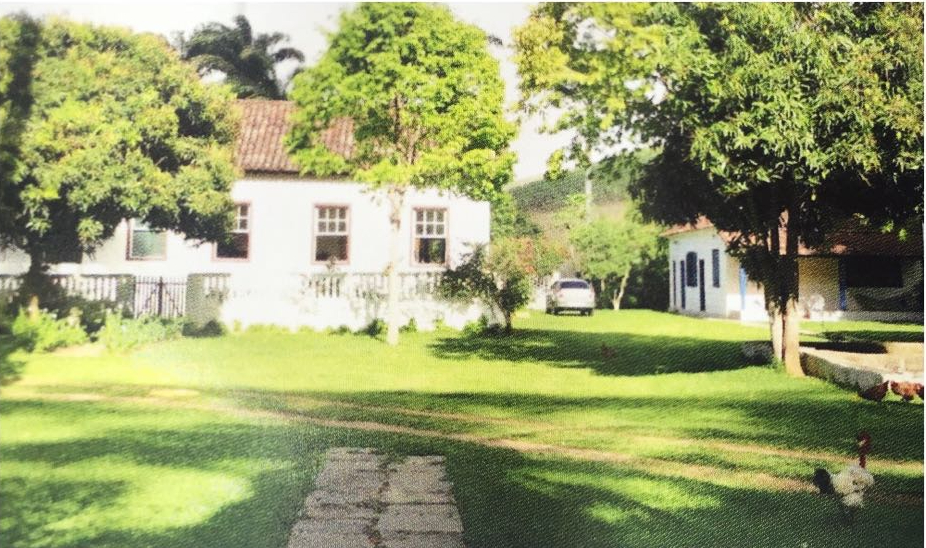
\includegraphics[scale=0.5]{entrance.jpeg}
		\caption{Entrance of the farm}
	\end{figure}
	\begin{figure}[H]
		\centering
		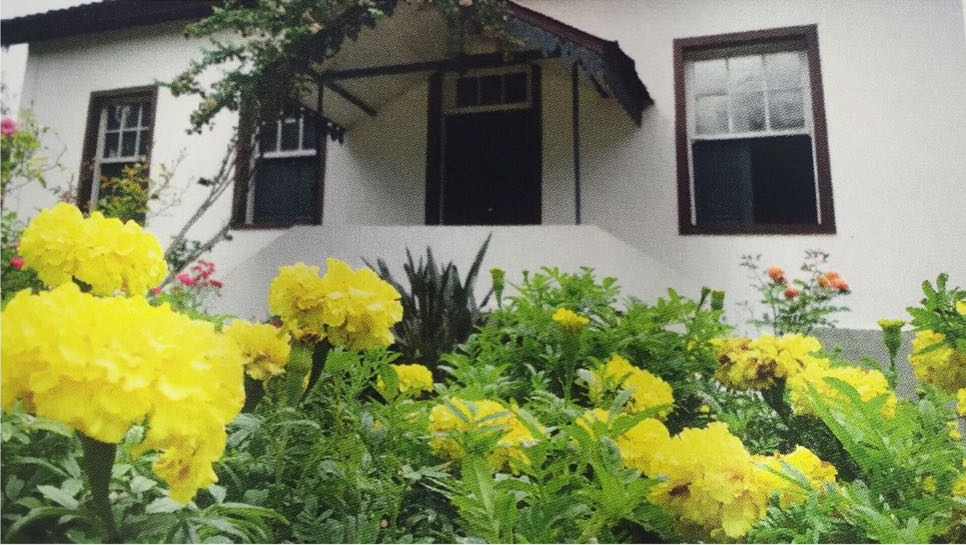
\includegraphics[scale=0.42]{flowers.jpeg}
		\caption{Flowers in the house garden}
	\end{figure}
	\begin{figure}
		\centering
		\begin{minipage}{.5\textwidth}
			\centering
			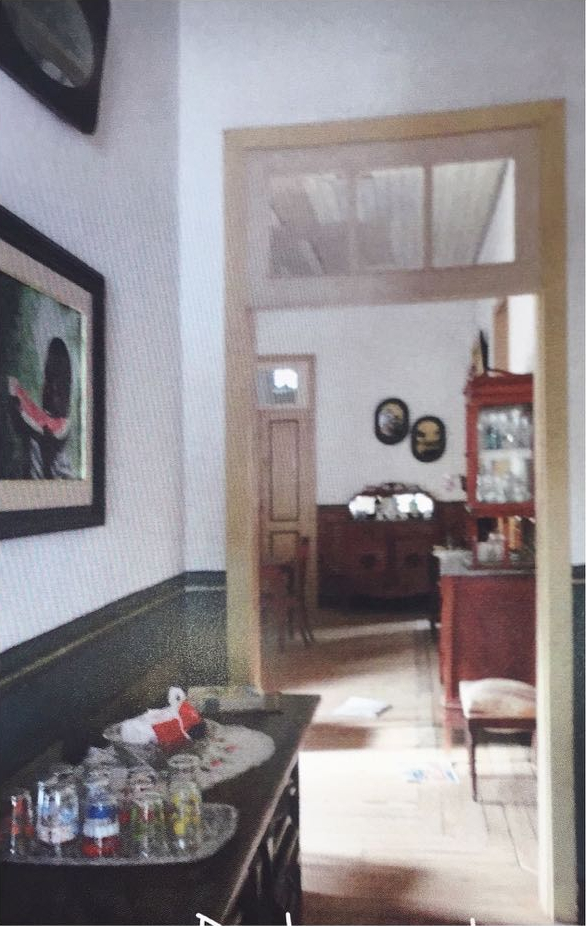
\includegraphics[width=\linewidth]{hall.jpeg}
			\captionof{figure}{Hall of the house}
		\end{minipage}%
		\begin{minipage}{.5\textwidth}
			\centering
			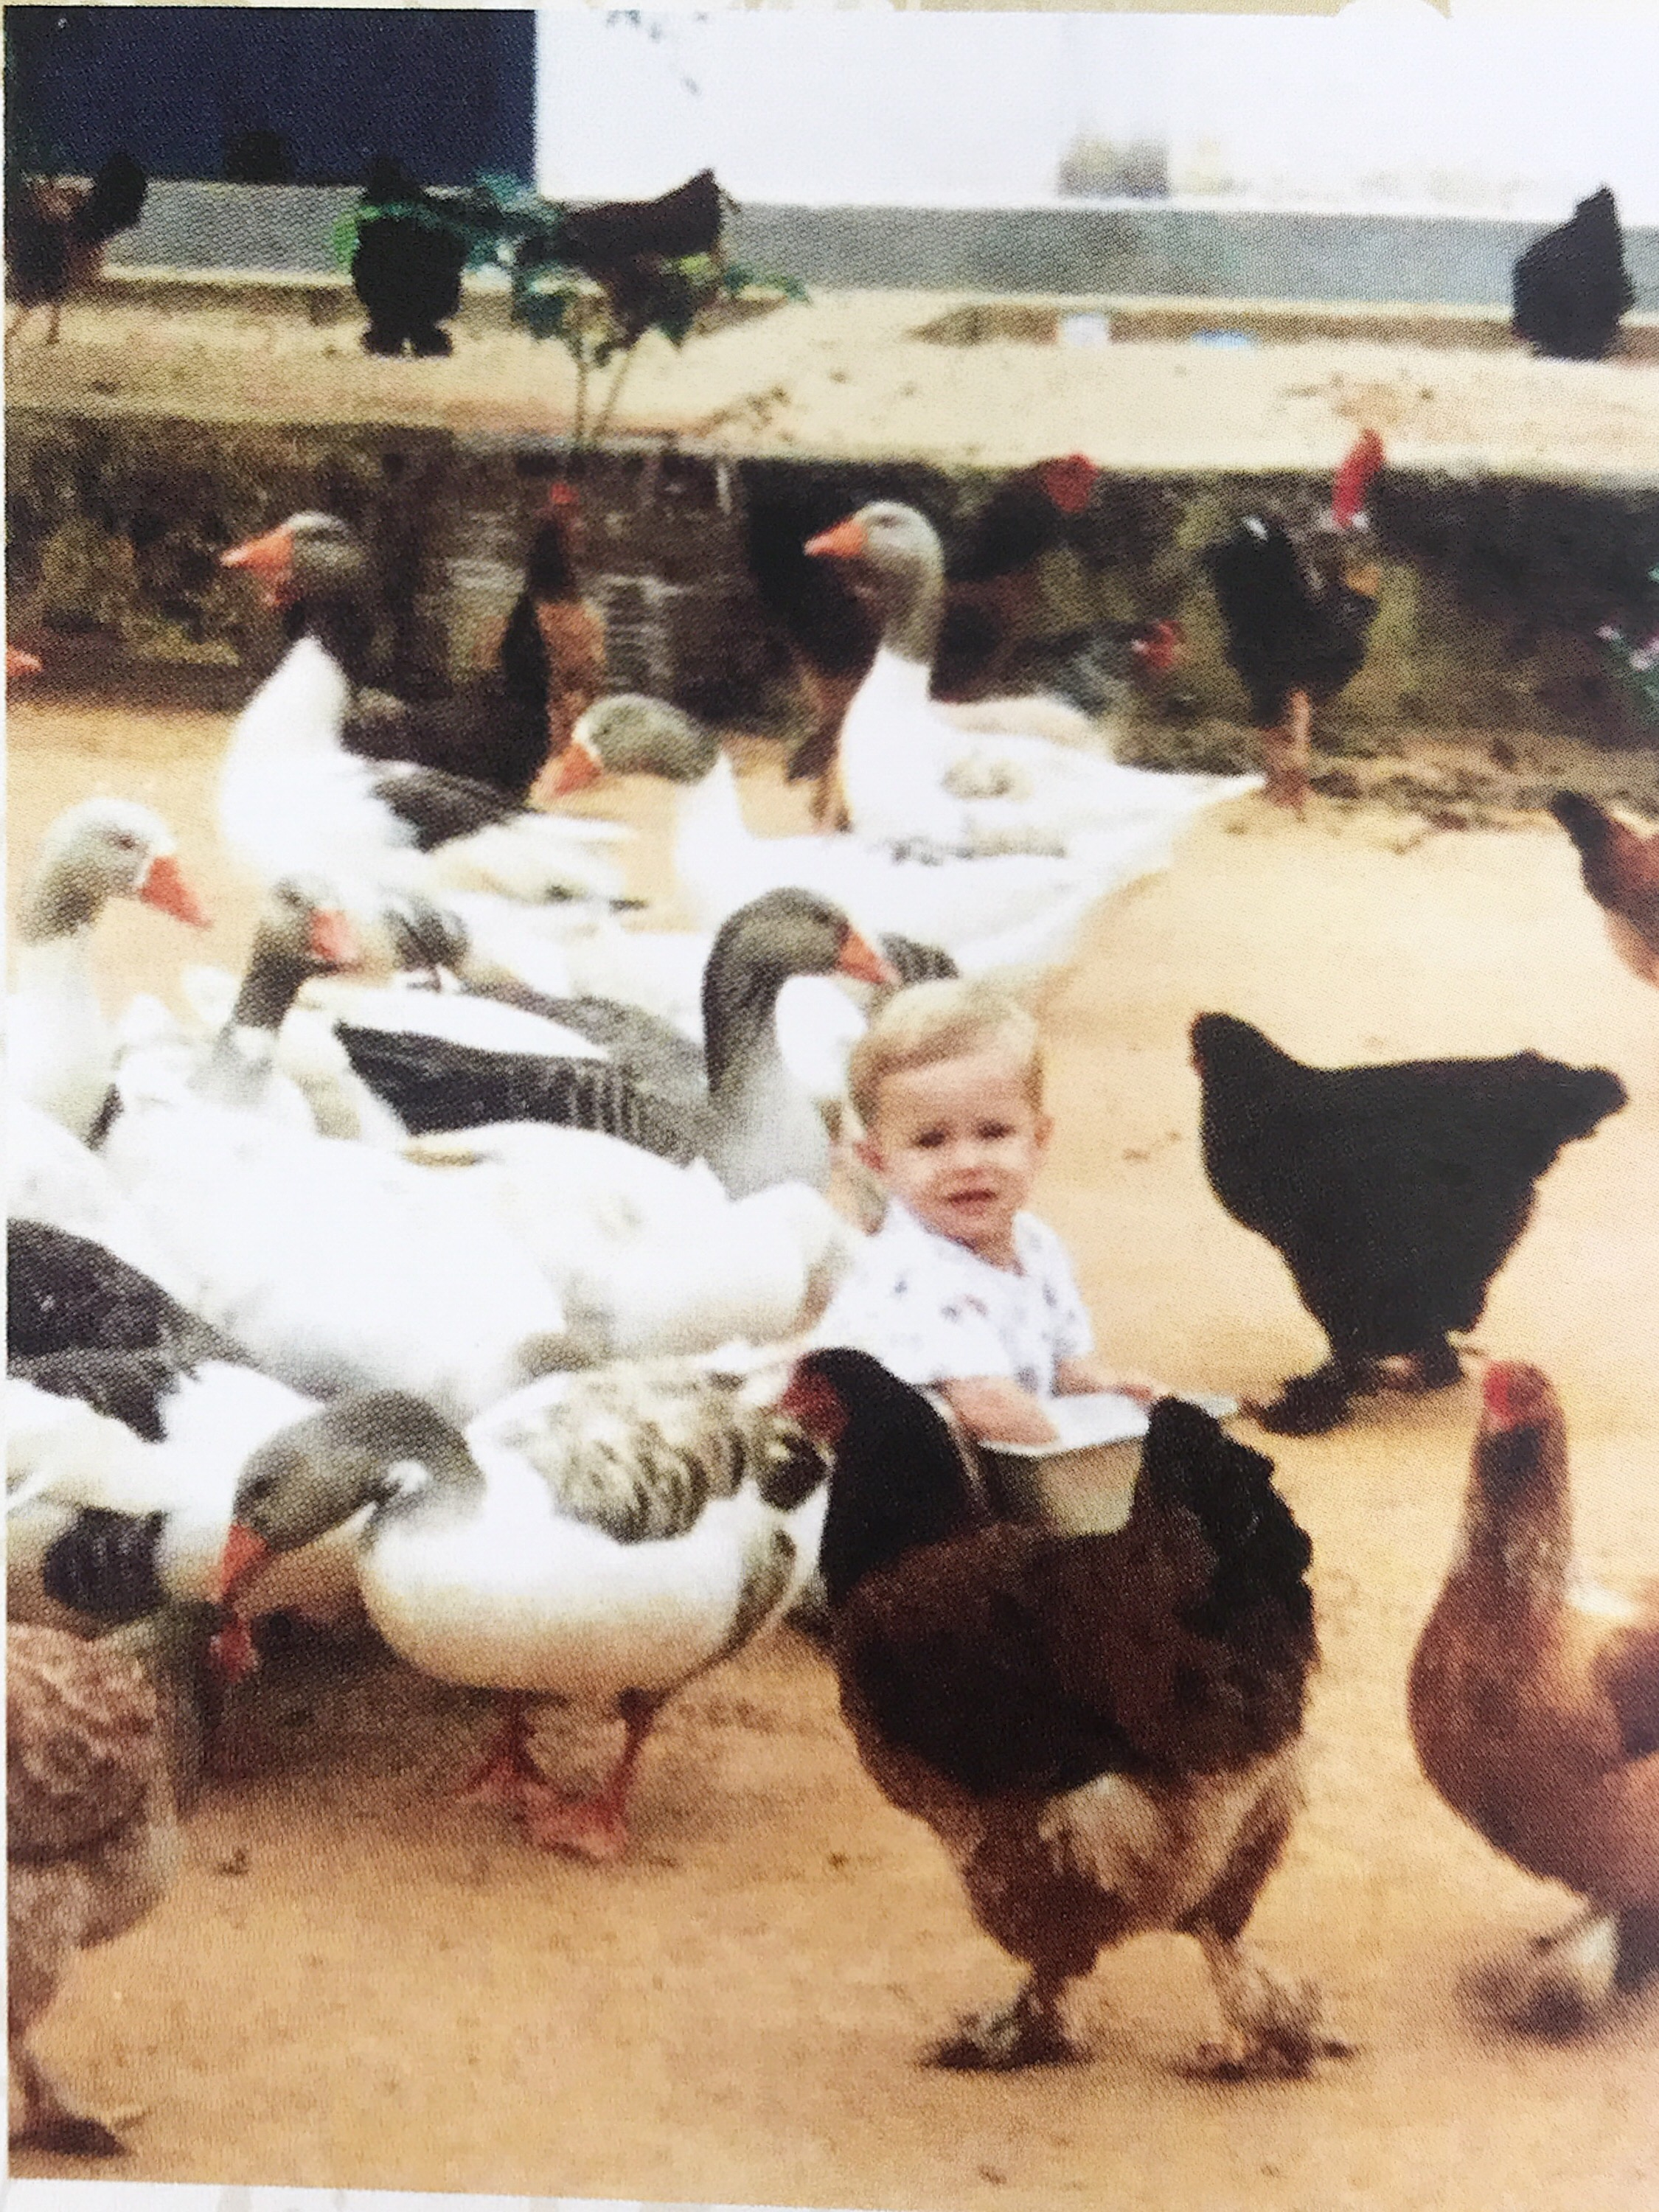
\includegraphics[width=\linewidth]{chickens.jpg}
			\captionof{figure}{Me feeding the chicken}
		\end{minipage}
	\end{figure}

	\begin{figure}[H]
		\centering
		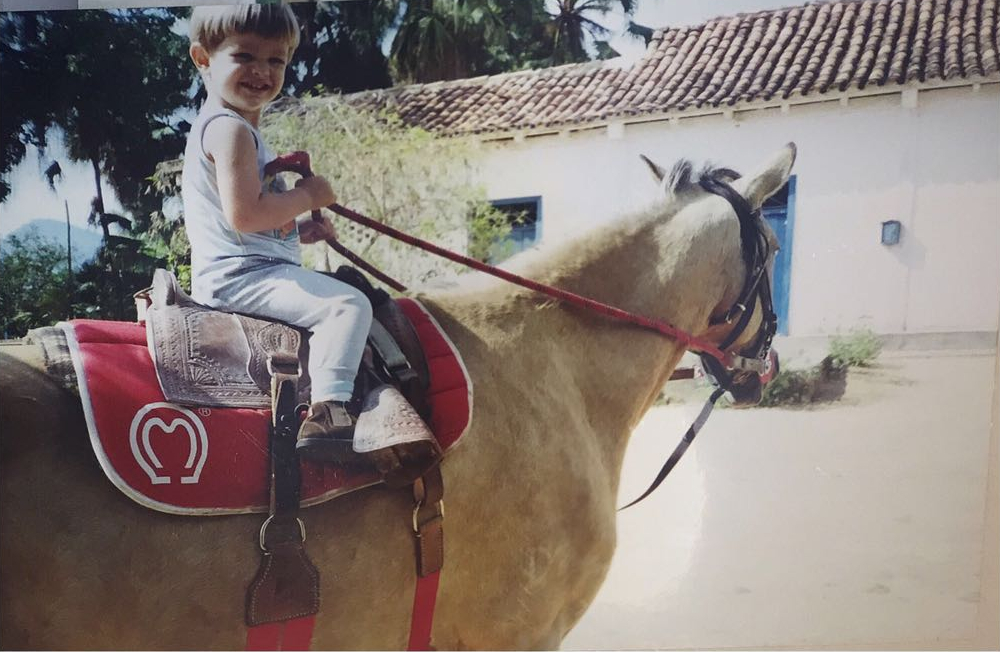
\includegraphics[scale=0.4]{horse.jpeg}
		\caption{Me learning to ride a horse}
	\end{figure}

	\newpage
	\vspace*{\fill}
	\begin{figure}[H]
		\centering
		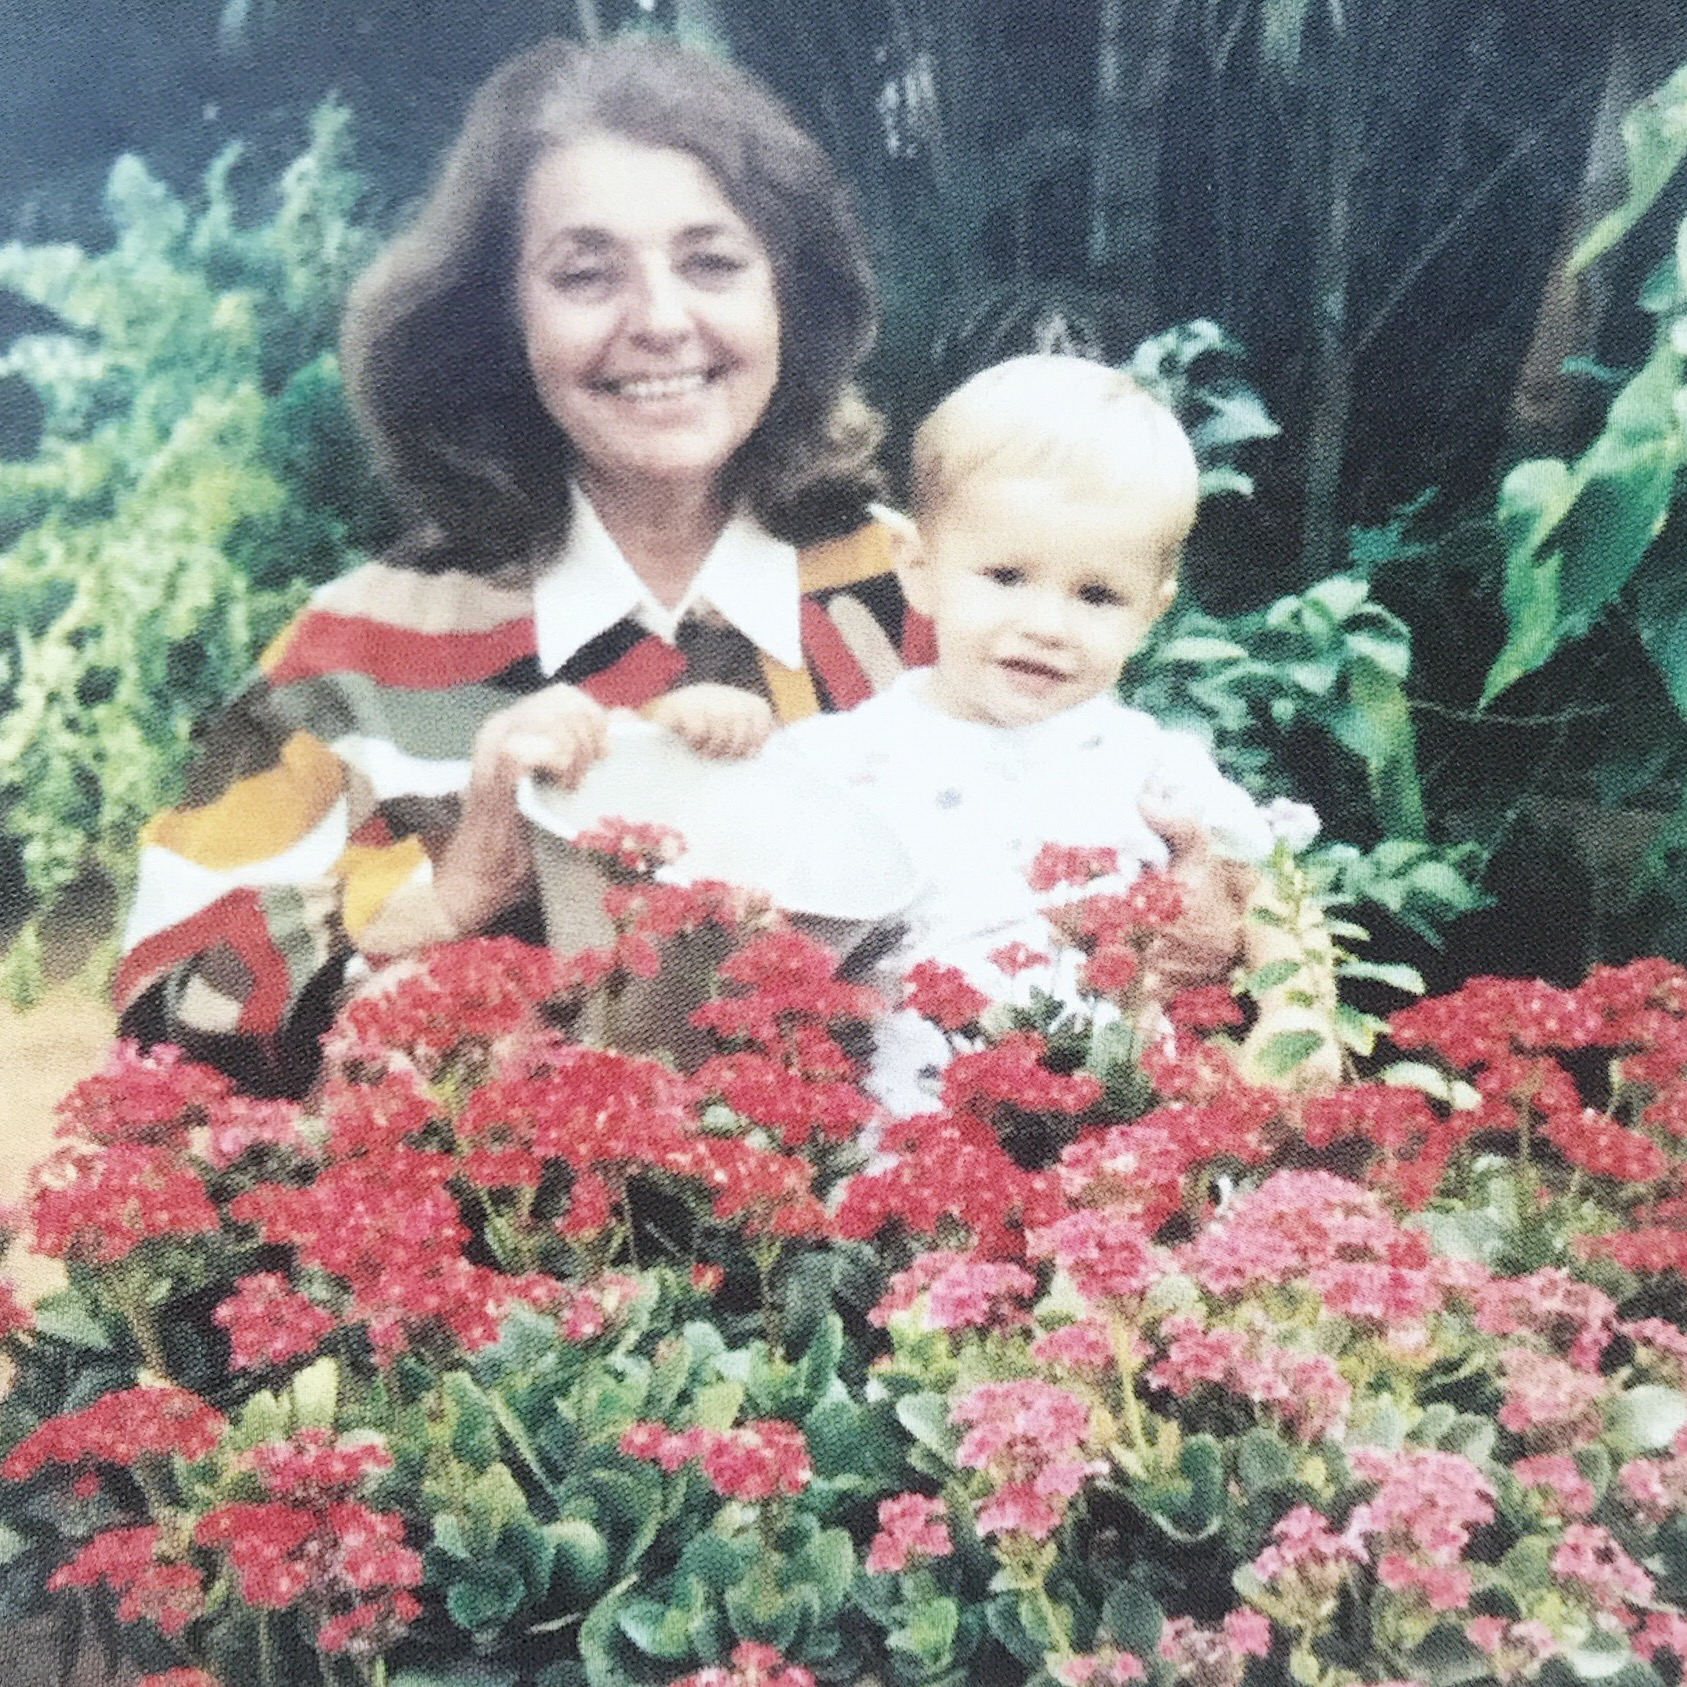
\includegraphics[width=\linewidth]{flowers-2.jpg}
		\caption{My great-aunt and I picking flowers}
	\end{figure}
	\vspace*{\fill}
	\newpage

	\section*{Appendix B}
	\begin{center}
		A life lived at random
	\end{center}
	\tab{} It was a painfully warm summer day in Rio. I know this may sound hyperbolic, but that is only the case if you haven't experienced Rio summer. When it's mid-January (inverted seasons, remember?) and the thermometers are hitting 120 ºF while humidity is at a sweet 90\%, it is hard to find someone who won't call it painful. And it was one of these days. I had taken the wrong bus accidentally on my way to the Makerspace I ran, which not only meant I had to walk further, but also that this line had no AC, which basically made the bus a sauna on wheels, sweat included.

	The traveling kiln dropped me off a couple blocks from my destination, in front of a bookstore. I probably wouldn't have noticed it, but they had themed their window with a variety of blue-colored books, and since I'm fond of blue, it caught my eye. The fact that they, unlike the bus, had AC made it an invitation to come inside, which I did, to refresh and dry if nothing else, which was when a book caught my eye. ``Quantum Theory by David Bohm,'' was written in the, blue, cover which featured a beautiful wave-like pattern in yellow and green. I didn't know who David Bohm was, nor did I care for Quantum anything, and I also didn't understand why a book in English about physics had ended up at an unsuspecting Brazilian bookstore, I assume because it was blue, but I bought it, because I liked the cover.

	After about a week of reading the blue book, which I only did because it cost way more then it should have and so I decided I might as well peruse it, I understood nothing. It had a lot of math, which I didn't care for quite honestly, and an offensive lack of figures for a book with such a pretty cover. Eventually, after much protraction, I read it through, and let it occupy my mind for a few days. I was in a bus, this time the right one, when it struck me: ``Will an n-dimensional being cause the superposition of a state not observable to his dimension to collapse on observation of a particle?'' Yes, I know it sounds like word-mush, but I promise there's a thread of sense in that question, and it fascinated me, and most importantly I had no idea what the answer was.

	It took a bit of poking around the internet, but eventually I found a Physics chat, which a bunch of people who knew Quantum Mechanics to tell me how my question was wrong. It so happens that it was quite late when I decided to ask my question on the chat, late enough in Brazil for it to be about time someone from California might be getting home from work. While two Germans taunted me about not understanding something I don't remember, one user called Daniel took his time in talking to me about the question, and explaining it.

	In the following months me and Daniel started talking, and became friends. I visited him later that year, and then again to attend his wedding, and we never really stopped talking. Afterwards, when I felt like I had to leave Lisbon before I turned my partial lunacy into complete dissociation with reality, Daniel suggested I come to Santa Barbara, and then, as we say in Portuguese, the rest is history.

	This story, which is entirely real furnace-bus and all, is just one example of how unlikely, how chaotic, reality is; there are many others. I only know my girlfriend because I picked a random class last semester; I only know my housemates because our papers got switched during orientation; I only ended up in Lisbon because I got a good grade at my high school exit exam essay (which in Brazil is pretty much just dumb luck); I only chose mathematics because I got a book, ``Gentle Art of Mathematics,'' from eBay because I liked the title. The point being, life is this amazingly intricate tapestry of unlikely events, and I think to look back and realize that is absolutely awe inspiring.

	In a way, I think this is what Mitchell is getting at in Ghostwritten, how people's lives are interwoven in unlikely and unpredictable ways. By and large all those characters are thoroughly different people, in distantly different conditions and places, and yet their lives and stories are subtly sown together. Perhaps this is what Ghostwritten, the title itself, refers to: an allusion to some higher being, ghostwriting the stories of our lives.

	In Lion we see this same unlikely tapestry being woven together. Saroo is lost because he decides on a whim to follow his brother. He gets on a train that could go anywhere. He escapes the kidnappers at the train station by luck. A cascade of events lead him to meet the young man at the café who takes him to the police. He is selected, from thousands of children, to be adopted by that specific family, and so on. Every particular aspect of reality is, when looked at carefully, so unlikely.

	I think the wisdom to be taken from Ghostwritten and Lion, from a certain perspective, is that the beauty, in a truly aesthetic sense, of life is not related to whether things do or don't go well, or as expected. The beauty of life is life in and of itself, it's the cascade of almost-impossibly unlikely events that compose life. Whether or not life is what we'd like it to be doesn't really have a bearing here, it's beautiful because it exists.
\end{mla}
\end{document}